\chapter{Requirements and Architecture}\label{cha:requirements_and_architecture}\thispagestyle{fancy}
\section{Introduction}\label{sec:introduction}
\subsection{Structure of the Document}\label{sec:structure_of_document}
This chapter is a collection of the thoughts that went into the design and development of version 1 of the system. The document
also functions as a documentation of the smallest set of functionalities and requirements that make up the developed application.
Chapter~\ref{cha:sprint_and_backlog_documentation} will contain a documentation of which requirements were implemented by which
ticket and with which version. It will also server as a backlog and reference over the tickets that should be done in a given
development cycle. More on the specific development workflow in said chapter.

The following section will give an overview over the context (subsection~\ref{sec:context_and_motivation}) and goals
(subsection~\ref{sec:goals_of_the_project}) of the project. Section~\ref{sec:requirements_engineering} will list the requirements 
of the developed application and will give an overview over the 

\subsection{Context and Motivation}\label{sec:context_and_motivation}
The fencing department of the local sports club provides equipment for kids and adults. This allows for newcomers to enjoy the
sport without buying the expensive equipment without knowing how they will like the sport and whether or not they want to 
keep fencing. This equipment is not maintained by any special party and will sometimes go months without proper testing and 
maintenance. As members change frequently and the armourer is not a fixed position in the ranks of the club there is no
comprehensive list or overview over the equipment and its working status. This is especially problematic when new fencers need
to borrow equipment from the club to compete in their first tournaments.

To solve the lacking-overview-problem, a system will be developed to assign unique identifiers to the weapons and keeping track of 
their condition. This task will be supported by a database holding the needed information.

\subsection{Goals of the project}\label{sec:goals_of_the_project}
The overarching goal is to develop a system that allows for keeping track over items present in a given inventory. In this context
these items are epees for fencing or equipment to setup the fencing piste. The goal is to be able to know who borrowed the weapon
and the working status of each item. The system should also facilitate the job of the armourer or the person currently in charge
of fixing the item, as the assessment of each weapon will simply be done already.

\subsection{Solution to the problem}\label{sec:problem_solution}
The solution for the problem presented in the previous section consists of two parts. At first, all epees in possession of the 
fencing department need to be collected and registerd. For that, each weapon is given a uinique identifier, which not only allows
to identify the weapon and make it storable in a computer based system, it allso will provide information about the weapon itself.
The ID will have three components: \#bs-h-id, where

\begin{itemize}
    \item $bs$ notes the size (length) of the blade. Technically, this can be any integer between 0 and 5, but for this
        project, only sizes 0 and 5 are needed.
    \item $h$ notes the handedness of the weapon, either left or right.
    \item $id$ is an ongoing number. It will increase for every new object registered in the database.
\end{itemize}

The index for every weapon needs to be created manually.

Secondly, the weapon is registered in a database, containing information about the status of the weapon, who currently owns it and
what maintenance has been done when and by whom. This database application is the subject of this document.

\section{Requirements Engineering}\label{sec:requirements_engineering}
\subsection{Requirements}\label{sec:requirements}
These requirements provide a foundation and minimal set of basic functionality of the application. Implicitly, this section also
servers as a documentation for the version v1.0.0 of the project and requirements for further versions of the project will contain
their own documentation. 

The section will be devided into \emph{Functional Requirements} (Table~\ref{tab:functional_requirements}) and \emph{Nonfunctional
Requirements} (Table~\ref{tab:nonfunctional_requirements}). Each requirement will have an identifier, a description and a
priority. \emph{Must Have Requirements} (MH) are non-negotiable and need to be implemented first, as they ensure the correct and
planned behaviour and functionality of the application. \emph{Should Have Requirements} (SHR) can be postproned in favour of a
MHR, but should be considered when implementing other requirements and features.  \emph{Nice To Have Requirements} NtHR are
negotiable and can be implemented at later point in time.  

\subsubsection{Functional Requirements}
\begin{table}[!ht]
    \centering
    \begin{tabular}{ | b{0.09\linewidth} | b{0.7\linewidth} | b{0.09\linewidth} | }
        \hline
        \textbf{ID} & \textbf{Description} & \textbf{Priority} \\
        FR01        & The application shall provide a database scheme to store weapon objects                   & MHR \\ \hline
        FR02        & The application shall implement the CRUD operations for every database scheme             & MHR \\ \hline
        FR03        & The application shall store the following information: ID of the weapon, current owner of the
                      weapon, a list of maintenance done on the weapon                                          & MHR \\ \hline
        FR04        & The application shall provide a mechanism to filter the list of results                   & SHR \\ \hline
        FR05        & The maintenance entry shall include the date of maintenance, the maintenance work done
                      and the maintainer                                                                        & MHR \\ \hline
        FR06        & The application shall provide a graphical user interface (GUI) to interact with
                      the database                                                                              & MHR \\ \hline 
    \end{tabular}
    \caption{Functional Requirements}
    \label{tab:functional_requirements}
\end{table}

\subsubsection{Nonfunctional Requirements}
\begin{table}[!ht]
    \centering
    \begin{tabular}{ | b{0.09\linewidth} | b{0.7\linewidth} | b{0.09\linewidth} | }
        \hline
        \textbf{ID} & \textbf{Description} & \textbf{Priority} \\
        \hline
        NFR01       & The application shall be constructed in such a way that new types of material can
                      easily added in the database                                                          & MHR \\ \hline
        NFR02       & Backend and frontend should not be coupled and be interchangable from oneanother      & MHR \\ \hline
    \end{tabular}
    \caption{Nonfunctional Requirements}
    \label{tab:nonfunctional_requirements}
\end{table}

\subsection{Architectural Design}\label{sec:architectural_design}
The following section defines the architecural design. The section the general idea behind the structure of the project and an
overview of the designchoises.

\subsubsection{Designoverview}

Figure~\ref{fig:architecural_overview} shows the design of the application. It follows the layer pattern,
which is used to decouple frontend from backend. There are three layers: The presentation layer, the API Layer and
the Data Access Layer. 

The presentation layer provides a GUI for the user to interact with the system and to display the data provided by the API.
The API layer defines endpoints which can be used by the frontend to request data from the database. It servers as a connector
which connects prensentationlayer and database. It uses components from the data access layer to forward the data requests from
the presentation layer. The data access layer defines the operations which can be done on the database.

\begin{figure}
    \centering
    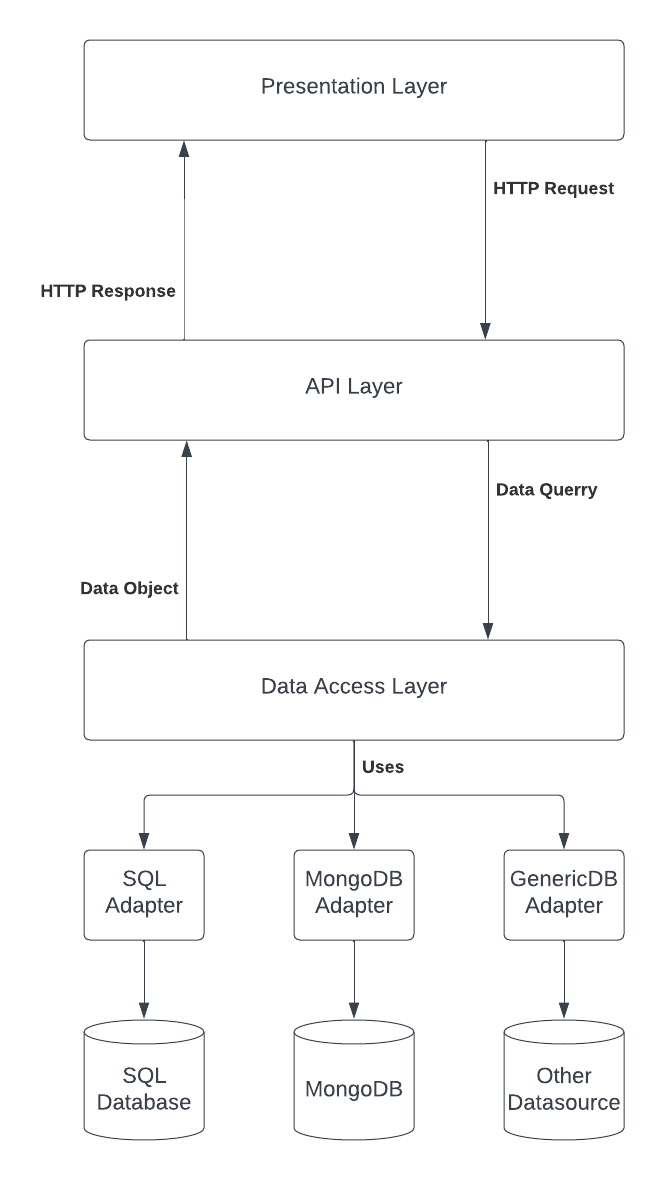
\includegraphics[scale=0.5]{IMG/amo_architecture}
    \caption{Archtecutral Overview of the AMO System}
    \label{fig:architecural_overview}
\end{figure}

The driving factor behind every descition made in the development process is the flexibility to adapt to future changes.  Because
the system is not yet tested and requirements were not gathered through user-centric processes, unforseen requirements can arise
in the future and during usage of the system. For this reason, the system was designed to be modular and flexible for change.  By
using the layer architecture, the system provides a modular way to change database and frontend technologies independant from
oneanother.

Database services should not be accessed driectly, as it should be possible to switch between technologies as needed. For this
reason, the data access layer defines data base adapters, which implement the specific querries for each database. The API should
only know of the classic CRUD operations (Create, Read, Update and Delete) and delegate, which to use when and with which
parameters.

\section{Languages and Frameworks}
The application will be written using the Python programming language. This is done for two reasons. First, performance is not
(yet) a requirement to be considered, and secondly it allows for rapid prototyping. As the first version of the amo system serves
as a proof of concept, the tradeoff {\glqq less performance for faster development\grqq} can be safely made. If at some point in
the future, performance will get an issue and a faster programming language will do the trick, then a switch can be made.

The framework of choise is Flask. Flask is a minimal backend framework for the Python language. It is used to provide the API
and handle requests / responses, routing, user authentication etc. Because of it simplicity it is flexible and allows the
developer to implement custom soulutions.
